\documentclass[11pt,reqno]{amsart}
\usepackage[T1]{fontenc}
\usepackage[utf8]{inputenc}
\usepackage{lmodern}
\usepackage{amsmath,amssymb,amsthm,microtype,etoolbox,needspace}
\usepackage[a4paper,hmargin=22.5mm,vmargin=22mm]{geometry}
\usepackage{tikz}
\definecolor{stripred}{HTML}{B84655}
\definecolor{stripblue}{HTML}{3477B9}
\makeatletter
\patchcmd{\@maketitle}{\global\topskip42\p@\relax}{\global\topskip18\p@\relax}{}{}
\patchcmd{\@maketitle}{\dimen@34\p@}{\dimen@26\p@}{}{}
\patchcmd{\@setauthors}{\@topsep30\p@\relax}{\@topsep20\p@\relax}{}{}
\makeatother
\usepackage[hidelinks]{hyperref}
\urlstyle{same}
\hypersetup{pdftitle={Sharp Favard decay with uniform marginals},
 pdfauthor={Sergiu Alexandru Bîsceanu},
 pdfsubject={A compact set of unit length with uniform coordinate marginals and optimal Favard decay},
 pdfkeywords={Favard length, uniform marginals, permutation strips, Kaczynski conjecture}}
\newtheorem{theorem}{Theorem}
\newtheorem{corollary}[theorem]{Corollary}
\newtheorem{lemma}{Lemma}
\newcommand{\Fav}{\operatorname{Fav}}
\newcommand{\supp}{\operatorname{supp}}
\newcommand{\E}{\mathbb E}
\newcommand{\A}{\mathcal A}
\newcommand{\R}{\mathbb R}
\setlength{\emergencystretch}{1.5em}
\setlength{\intextsep}{7pt plus 2pt minus 2pt}
\linespread{1.035}
\renewcommand{\bibliofont}{\normalfont\small}
\title{Sharp Favard decay with uniform marginals}
\author{Sergiu Alexandru B\^{\i}sceanu}
\date{}

\begin{document}
\begin{abstract}
For the $n$ parallelograms obtained by matching the equal subintervals of the
two horizontal edges of the unit square, we prove that the minimum area of
their union is of order $\frac1{\log n}$, as conjectured by Kaczynski.
\end{abstract}
\maketitle
\pagestyle{plain}
\raggedbottom
\widowpenalty=10000
\clubpenalty=10000

Divide the top and bottom edges of the unit square into $n$ equal intervals,
match them by a permutation, and join matched intervals by parallelograms.
Their areas add to $1$; the question is how small their union can be.
Writing $\alpha_n$ for the minimum, we call the assertion
$\alpha_n\asymp\frac{1}{\log n}$ \emph{KC2}.\footnote{KC2 abbreviates
``Kaczynski's Conjecture 2,'' following its numbering in
Kuklinski~\cite[\S\,3]{Kuklinski}.}

A strip joining $I$ to $J$ is encoded by the square $I\times J$ in the
plane of endpoints. At height $t$, its section is the projection
$\pi_t(I\times J)$, where $\pi_t(x,y)=(1-t)x+ty$.
A set with a unit coordinate projection has Hausdorff length at least $1$.
We attain this minimum with both coordinate projections equal to $[0,1]$,
together with a logarithmic bound on the averaged projections of its
neighborhoods.
For compact $S\subset\R^2$, put $S_\delta=S+[-\delta,\delta]^2$
and define its unnormalized Favard length by
\[
 \Fav(S)=\int_0^\pi|p_\theta(S)|\,d\theta,
 \qquad p_\theta(x,y)=x\cos\theta+y\sin\theta.
\]
Let $p_x,p_y$ be the coordinate projections. We write $|\cdot|$ for
length or area, and $\mathcal H^1$ for Hausdorff length.

\begin{theorem}\label{thm:favard}
There is a compact set $S\subset[0,1]^2$ such that
\[
 p_x(S)=p_y(S)=[0,1],\qquad \mathcal H^1(S)=1,
\]
and, for absolute constants $c,C>0$,
\[
 \frac{c}{\log \frac{1}{\delta}}\le\Fav(S_\delta)
 \le\frac{C}{\log \frac{1}{\delta}}\qquad(0<\delta<\frac{1}{2}).
\]
Its length measure $\mu=\mathcal H^1|_S$ has uniform coordinate marginals.
\end{theorem}

\begin{corollary}[KC2]\label{cor:kc2}
There is an absolute constant $C$ such that, for every $n\ge2$,
\[
 \frac1{H_n}\le\alpha_n\le\frac C{\log n},
 \qquad H_n=\sum_{j=1}^n\frac1j.
\]
\end{corollary}

The marginal condition means that
$\mu(B\times[0,1])=\mu([0,1]\times B)=|B|$ for Borel $B\subset[0,1]$.
A probability measure with these marginals is a \emph{permuton}~\cite{Permutons}.
In our construction, the marginal condition follows from length $1$.

Chang, Shmerkin and Suomala~\cite{CSS} obtain sharp Favard decay for
random Cantor sets. Cs\"ornyei and Suomala~\cite{CS} characterize the
measures which can occur as one projection of a purely unrectifiable
length measure. We require both marginals, together with the quantitative
bound. The fixed-base construction is too restrictive: for nested
$L$-adic permutation patterns, \cite[Theorem~A.1]{CSS} gives Favard length
$\gtrsim_L\frac{\log j}{j}$ at scale $L^{-j}$. We instead allow the widths of the
squares to vary.
Throughout, $c,C$ are positive absolute constants, allowed to change.

\Needspace{8\baselineskip}
\section{The matching reduction}

Length $1$ already forces the marginal condition. Indeed, suppose
$p_x(S)=p_y(S)=[0,1]$ and $\mathcal H^1(S)=1$, and put
$\mu=\mathcal H^1|_S$.
For either coordinate projection $p$ and Borel $B\subset[0,1]$,
the set $S\cap p^{-1}(B)$ projects onto $B$.
Since $p$ is $1$-Lipschitz, $\mu(p^{-1}(B))\ge|B|$.
The same inequality for the complement, together with total mass $1$,
forces equality.

Put $\A(S)=\int_0^1|\pi_t(S)|\,dt$.
The angular change of variables
$t=\frac{\sin\theta}{\cos\theta+\sin\theta}$ gives
\begin{equation}\label{eq:angular}
 \A(S)=\int_0^{\frac{\pi}{2}}
 \frac{|p_\theta(S)|}{(\cos\theta+\sin\theta)^3}\,d\theta
 \le\Fav(S).
\end{equation}

Let $\mu$ have uniform coordinate marginals and be supported on $S$.
Partition $[0,1]$ into $n$ intervals $I_i$ of length $\frac{1}{n}$,
half-open except for the last, which includes $1$.
The matrix $a_{ij}=n\mu(I_i\times I_j)$ has every row sum and column
sum equal to $1$. Any $k$ rows have total mass $k$ and therefore meet
at least $k$ columns, since each column has mass $1$.
This is Hall's condition, so the matching theorem~\cite{Hall} supplies
a permutation $\sigma$ with $a_{i,\sigma(i)}>0$ for all $i$.
Every selected cell meets $S$, so, closing the cells,
\begin{equation}\label{eq:matching}
 P_\sigma:=\bigcup_{i=1}^n
 \overline I_i\times\overline I_{\sigma(i)}\subset S_{\frac{1}{n}}.
\end{equation}
The slice of the associated strip union at height $t$ is
$\pi_t(P_\sigma)$. Thus the upper bound in Theorem~\ref{thm:favard}
implies the corollary through
\begin{equation}\label{eq:reduction}
 \alpha_n\le\A(P_\sigma)\le\A(S_{\frac{1}{n}})
 \le\Fav(S_{\frac{1}{n}})\le\frac C{\log n}.
\end{equation}
For $n=2$, increase $C$ if necessary.

The lower bound is a pairwise overlap count. In any permutation-strip
arrangement of area $A$, let $Z$ count the strips covering a point.
Then $\int Z=1$ and Cauchy--Schwarz gives $1\le A\int Z^2$.
Two crossing strips with endpoint index gaps $p,q\ge1$ have
intersection area
\[
 \frac1{n(p+q)}\le\frac1{4n}\left(\frac1p+\frac1q\right).
\]
Their signed displacement is $\frac{p-(p+q)t}{n}$, so the overlap length
has a triangular graph of height $\frac{1}{n}$ and base $\frac{2}{p+q}$.
Noncrossing pairs have no positive-area intersection.
On either edge there are $n-d$ pairs of index gap $d$.
Counting each pair twice in $Z^2$ therefore gives
\begin{equation}\label{eq:lower}
 \int Z^2\le1+\frac1n\sum_{d=1}^{n-1}\frac{n-d}{d}=H_n,
 \qquad A\ge\frac1{H_n}.
\end{equation}
For any uniform-marginal measure, take $n=\lceil\frac{1}{\delta}\rceil$ in
\eqref{eq:matching}. Since $\frac{1}{n}\le\delta$, equations
\eqref{eq:angular} and \eqref{eq:lower} give
$\Fav(S_\delta)\ge\A(P_\sigma)\ge\frac{1}{H_n}\ge \frac{c}{\log \frac{1}{\delta}}$.
Thus the Favard lower bound holds for every compact set carrying a
probability measure with uniform marginals. We now construct a set
attaining it with length $1$.

\section{Finite patterns}

A \emph{pattern} is a set
$P=\bigcup_{i=1}^N(I_i\times J_i)$, where each family of closed intervals $(I_i)$ and $(J_i)$ covers
$[0,1]$ with disjoint interiors, and $|I_i|=|J_i|=w_i>0$. Write $N(P)$ for its number of squares. The sum of their sides is $1$.

A red--blue shuffle preserves both interval partitions while reducing
projection length. We also control the number of squares: thickening
$N$ squares by $\delta$ costs at most $CN\delta$ in Favard length.

\begin{lemma}[Finite patterns]\label{lem:compression}
For every integer $k\ge1$ there is a pattern $P$ such that
\[
 \Fav(P)\le \frac{C}{k},\qquad \log N(P)\le Ck.
\]
\end{lemma}

\begin{proof}
Each shuffle will give a quadratic expected saving in Favard length
at bounded expected cost in $\log N$.
Given a pattern $P$, write $E_t=\pi_t(P)$, $\ell(t)=|E_t|$ and
$L(P)=\int_0^{\frac{1}{2}}\ell(t)\,dt$.
We first estimate the overlap for $0\le t\le\frac{1}{2}$.

Choose a width $0<w<1$ and partition a unit interval
into $m=\lceil\frac{1}{w}\rceil$ pieces of width $w$, with the last possibly
shorter. Take red and blue copies of this partition, and place them on
coordinate intervals of length $2$ in the orders
\begin{equation}\label{eq:orders}
 \begin{array}{rl}
 x\text{-axis}:&R_1,B_1,R_2,B_2,\ldots,R_m,B_m,\\
 y\text{-axis}:&B_1,B_2,\ldots,B_m,R_1,R_2,\ldots,R_m.
 \end{array}
\end{equation}
Equal labels determine squares. Put a homothetic copy of $P$ inside each
square, then divide both coordinates by $2$. The resulting pattern $P_w$
has $MN(P)$ squares, where $M=2m$. Its copy ratios sum to $1$, so
subadditivity gives $|\pi(P_w)|\le|\pi(P)|$ for every linear projection $\pi$.

% Exact w=1/2 shuffle, with the 132 pattern in each copy.
% All coordinates are affine images of the same twelve endpoint squares.
% The first matched pair is emphasized in every panel.
\begin{figure}[htbp]
\centering
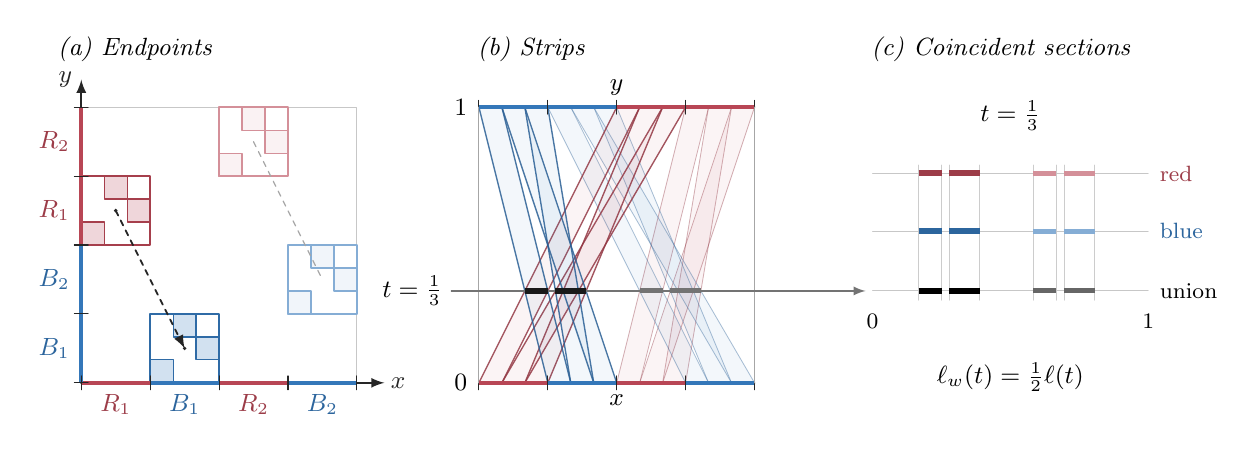
\begin{tikzpicture}[x=1cm,y=1cm,>=latex,
  every node/.style={font=\small},line cap=round,line join=round]
% (a) Four copies of the same 132 pattern, with the first pair in the foreground.
\begin{scope}[x=3.5cm,y=3.5cm]
\node[anchor=west] at (-.12,1.21) {\textit{(a) Endpoints}};
\draw[black!22,line width=.35pt] (0,1)--(1,1)--(1,0);
\foreach \a/\b/\col/\ink/\tint in
 {0/.5/stripred/stripred!90!black/22,.25/0/stripblue/stripblue!90!black/22,.5/.75/stripred/stripred!60/7,.75/.25/stripblue/stripblue!60/7}{
  \foreach \u/\v in {0/0,1/2,2/1}{
    \path[fill=\col!\tint,draw=\ink,line width=.45pt]
      ({\a+\u/12},{\b+\v/12})
      rectangle ({\a+(\u+1)/12},{\b+(\v+1)/12});
  }
  \draw[\ink,line width=.65pt] (\a,\b)
    rectangle ({\a+.25},{\b+.25});
}
% The translation from red to blue is in ker pi_{1/3}.
\draw[->,black!86,dash pattern=on 2pt off 2pt,line width=.65pt]
  (.125,.625)--(.375,.125);
\draw[black!35,dash pattern=on 2pt off 2pt,line width=.45pt]
  (.625,.875)--(.875,.375);
\foreach \a/\b in {.125/.625,.375/.125}{
  \fill[black!85] (\a,\b) circle[radius=.7pt];
}
\draw[->,black!85,line width=.65pt] (0,0)--(1.10,0)
  node[right,inner sep=2pt] {$x$};
\draw[->,black!85,line width=.65pt] (0,0)--(0,1.10)
  node[left,inner sep=3pt] {$y$};
\foreach \a/\col/\lab in {0/stripred/R_1,.25/stripblue/B_1,.5/stripred/R_2,.75/stripblue/B_2}{
  \draw[\col,line width=1.6pt,line cap=butt] (\a,0)--({\a+.25},0);
  \node[below,inner sep=4pt,text=\col!85!black] at ({\a+.125},0) {$\lab$};
}
\foreach \a/\col/\lab in {0/stripblue/B_1,.25/stripblue/B_2,.5/stripred/R_1,.75/stripred/R_2}{
  \draw[\col,line width=1.6pt,line cap=butt] (0,\a)--(0,{\a+.25});
  \node[left,inner sep=4pt,text=\col!85!black] at (0,{\a+.125}) {$\lab$};
}
\foreach \a in {0,.25,.5,.75,1}{
  \draw[black!85,line width=.4pt] (\a,-.025)--(\a,.025);
  \draw[black!85,line width=.4pt] (-.025,\a)--(.025,\a);
}
\end{scope}
% (b) Exact strips, drawn back to front to keep the chosen pair legible.
\begin{scope}[xshift=5.05cm,x=3.5cm,y=3.5cm]
\node[anchor=west] at (-.04,1.21) {\textit{(b) Strips}};
\foreach \a/\b/\col/\opacity/\width in
 {.5/.75/stripred/.40/.3,.75/.25/stripblue/.40/.3,0/.5/stripred/.85/.5,.25/0/stripblue/.85/.5}{
  \foreach \u/\v in {0/0,1/2,2/1}{
    \path[fill=\col,fill opacity=.06,draw=\col!80!black,
      draw opacity=\opacity,line width=\width pt]
      ({\a+\u/12},0)--({\a+(\u+1)/12},0)--
      ({\b+(\v+1)/12},1)--({\b+\v/12},1)--cycle;
  }
}
\draw[black!85,line width=.65pt] (0,0)--(1,0) (0,1)--(1,1);
\foreach \a/\col in {0/stripred,.25/stripblue,.5/stripred,.75/stripblue}{
  \draw[\col,line width=1.6pt,line cap=butt] (\a,0)--({\a+.25},0);
}
\foreach \a/\col in {0/stripblue,.25/stripblue,.5/stripred,.75/stripred}{
  \draw[\col,line width=1.6pt,line cap=butt] (\a,1)--({\a+.25},1);
}
\foreach \a in {0,.25,.5,.75,1}{
  \draw[black!85,line width=.4pt] (\a,-.025)--(\a,.025);
  \draw[black!85,line width=.4pt] (\a,.975)--(\a,1.025);
}
\draw[black!35,line width=.35pt] (0,0)--(0,1) (1,0)--(1,1);
\draw[black!55,line width=.45pt] (-.10,1/3)--(1.08,1/3);
\node[left,inner sep=3pt] at (-.10,1/3) {$t=\frac13$};
% Exact components: first pair dark, second pair pale.
\draw[black!90,line width=2.2pt,line cap=butt] (1/6,1/3)--(1/4,1/3);
\draw[black!90,line width=2.2pt,line cap=butt] (5/18,1/3)--(7/18,1/3);
\draw[black!55,line width=1.8pt,line cap=butt] (7/12,1/3)--(2/3,1/3);
\draw[black!55,line width=1.8pt,line cap=butt] (25/36,1/3)--(29/36,1/3);
\node[left,inner sep=4pt] at (0,1) {$1$};
\node[left,inner sep=4pt] at (0,0) {$0$};
\node[below,inner sep=4pt] at (.5,0) {$x$};
\node[above,inner sep=4pt] at (.5,1) {$y$};
\end{scope}
% The same section is carried to the separated tracks, at the same height.
\draw[->,black!55,line width=.5pt]
  (8.83,{3.5/3})--(9.96,{3.5/3});
% (c) Complete color sections; the first paired overlap remains emphasized.
\begin{scope}[xshift=10.05cm,x=3.5cm,y=3.5cm]
\node[anchor=west] at (-.04,1.21) {\textit{(c) Coincident sections}};
\node at (.5,.97) {$t=\frac13$};
\foreach \a in {1/6,1/4,5/18,7/18,7/12,2/3,25/36,29/36}{
  \draw[black!20,line width=.35pt] (\a,.30)--(\a,.79);
}
\foreach \h/\col/\lab in {.76/stripred/\mathrm{red},.55/stripblue/\mathrm{blue},.333333/black/\mathrm{union}}{
  \draw[black!22,line width=.35pt] (0,\h)--(1,\h);
  \node[right,inner sep=4pt,text=\col!85!black,font=\footnotesize] at (1,\h) {$\lab$};
  \draw[\col!85!black,line width=2.1pt,line cap=butt] (1/6,\h)--(1/4,\h);
  \draw[\col!85!black,line width=2.1pt,line cap=butt] (5/18,\h)--(7/18,\h);
  \draw[\col!60,line width=1.8pt,line cap=butt] (7/12,\h)--(2/3,\h);
  \draw[\col!60,line width=1.8pt,line cap=butt] (25/36,\h)--(29/36,\h);
}
\node[below,inner sep=2pt,font=\footnotesize] at (0,.27) {$0$};
\node[below,inner sep=2pt,font=\footnotesize] at (1,.27) {$1$};
\node at (.5,.02) {$\ell_w(t)=\frac12\ell(t)$};
\end{scope}
\end{tikzpicture}
\caption{The shuffle for $w=\frac12$. Each labeled square contains the
same three-square pattern; the first red--blue pair is emphasized.
Its translation follows a fiber of $\pi_{\frac13}$, so the paired copies
have identical sections at $t=\frac13$. In (c), the red and blue sections are drawn separately;
their union is the section in (b).}
\label{fig:shuffle}
\end{figure}


Within either color, the enclosing squares occur in the same order on
both axes, so their $\pi_t$-projections have disjoint interiors.
Each color contributes exactly $\frac{\ell(t)}{2}$. Thus, writing
$\ell_w(t)=|\pi_t(P_w)|$, we have $\ell_w(t)\le\ell(t)$,
and the difference is the overlap between the colors.

\Needspace{7\baselineskip}
For a full-width pair, blue starts $w$ to the right of red on the
$x$-axis and one unit to its left on the $y$-axis, before scaling.
The projected displacement, in units of their common side, is
$d_w(t)=(1-t)-\frac{t}{w}$.
The full-width pieces occupy at least half of each unit partition.
Their red squares therefore have total side length at least $\frac{1}{4}$ after
scaling. Adding the overlaps with their blue partners gives
\begin{equation}\label{eq:overlap}
 \ell(t)-\ell_w(t)\ge\frac14
 \left|E_t\cap\left(E_t+d_w(t)\right)\right|.
\end{equation}
There is no overcounting because the red projections have disjoint interiors.

Averaging over translations makes the overlap depend only on length:
for measurable $E\subset[0,1]$, Fubini gives~\cite{Tao}
\begin{equation}\label{eq:convolution}
 \int_{\mathbb R}|E\cap(E+s)|\,ds=|E|^2.
\end{equation}
The integral counts the pairs in $E\times E$. Its integrand is even
and vanishes outside $[-1,1]$.

For $0<t\le\frac{1}{2}$, a negative shift $d_w(t)=-s$,
$0\le s\le1$, requires $w=\frac{t}{1-t+s}\asymp t$.
Small heights need small widths, so we sample
$w=U^2$, with $U$ uniform on $(0,1)$. Then
\[
 U=\sqrt{\frac{t}{1-t+s}},\qquad
 |dU|=\frac{\sqrt t}{2(1-t+s)^{\frac{3}{2}}}\,ds\gtrsim\sqrt t\,ds.
\]
These values lie in $(0,1]$. Evenness and \eqref{eq:convolution} give
$\E_w[\ell(t)-\ell_w(t)]\gtrsim\sqrt t\,\ell(t)^2$.
The square law gives an integrable reciprocal weight:
$\int_0^{\frac12}\frac{dt}{\sqrt t}<\infty$.
Weighted Cauchy--Schwarz gives
\begin{equation}\label{eq:drift}
 \E_w[\A(P)-\A(P_w)]\gtrsim
 \int_0^{\frac{1}{2}}\sqrt t\,\ell(t)^2\,dt
 \gtrsim\left(\int_0^{\frac12}\ell(t)\,dt\right)^2=L(P)^2.
\end{equation}

Since the weight in \eqref{eq:angular} is at most $1$, the saving in
Favard length is at least the saving in $\A$.

To cover all directions, let $T(x,y)=(y,x)$ and $R(x,y)=(x,1-y)$,
and first choose $G$ uniformly from $\{I,T,R,T\circ R\}$.
The map $T$ exchanges $t$ and $1-t$, while $R$ supplies the other angular
quadrant. Hence
\begin{equation}\label{eq:sectors}
 \sum_G L(GP)=\A(P)+\A(RP)\asymp\Fav(P).
\end{equation}
\Needspace{4\baselineskip}
Apply the shuffle to $GP$. Favard length is invariant under $G$;
averaging \eqref{eq:drift} and using Cauchy--Schwarz in
\eqref{eq:sectors} gives the quadratic saving
\[
 \E[\Fav(P)-\Fav((GP)_w)]\ge c\Fav(P)^2.
\]
Each shuffle multiplies the number of squares by $M$, so its contribution
to $\log N$ is $\log M$. Since
$M=2\lceil\frac{1}{w}\rceil\le\frac{4}{w}=\frac{4}{U^2}$,
$\E\log M\le\log4+2\int_0^1\log\frac{1}{u}\,du<\infty$.

Starting with the unit square, use fresh independent choices of $G,U$
at each of $k$ steps. Let $F_k,N_k$ be the
resulting Favard length and number of squares, and put $f_k=\E F_k$.
Conditional expectation and Jensen's inequality yield
\[
 f_{k+1}\le f_k-cf_k^2,\qquad
 f_k\le\frac{4}{1+4ck},\qquad \E\log N_k\le Ck.
\]
Here $f_0=4$, and $\frac{1}{f_{k+1}}\ge\frac{1}{f_k}+c$ proves the middle bound.
To obtain both bounds for the same pattern, use their normalized sum:
$\E[kF_k+\frac{\log N_k}{k}]\le C$.
Some realization has this sum at most $C$; since both terms are
nonnegative, it satisfies both estimates in the lemma.
\end{proof}

In particular, choosing $k$ of order $2^j$ supplies patterns $P_j$ with
\begin{equation}\label{eq:blocks}
 \Fav(P_j)\le2^{-j},\qquad \log N(P_j)\le C2^j.
\end{equation}

\Needspace{5\baselineskip}
\section{The limiting set}

To nest patterns, insert a copy of $Q$ into each square of
$P=\bigcup_i(v_i+w_i[0,1]^2)$:
\[
 P\star Q=\bigcup_i(v_i+w_iQ).
\]
The result is again a pattern, with $N(P)N(Q)$ squares. Moreover,
$P\star Q\subset P$, while $\sum_iw_i=1$ gives, for every linear
projection $\pi$,
\begin{equation}\label{eq:composition}
 |\pi(P\star Q)|\le
 \min\{|\pi(P)|,|\pi(Q)|\}.
\end{equation}

The squares of a pattern have total diameter $\sqrt2$. To obtain length
$1$, we group smaller squares inside copies of a pattern whose diameter
is close to $1$. For even $m$, let $B_m$
be the equal-grid pattern given by the cyclic half-shift
$i\mapsto i+\frac{m}{2}\pmod m$. It lies in the diamond
\[
 |x-\frac12|+|y-\frac12|\le\frac12+\frac1m.
\]
The diamond has diameter $1+\frac{2}{m}$, so
\begin{equation}\label{eq:buffer}
 \operatorname{diam}B_m\le1+\frac{2}{m}.
\end{equation}
Thus insertion into $B_m$ preserves the projection bound and gives a
cover of diameter tending to $1$.

% Exact vector geometry. No TikZ libraries are required.
\begin{figure}[htbp]
\centering
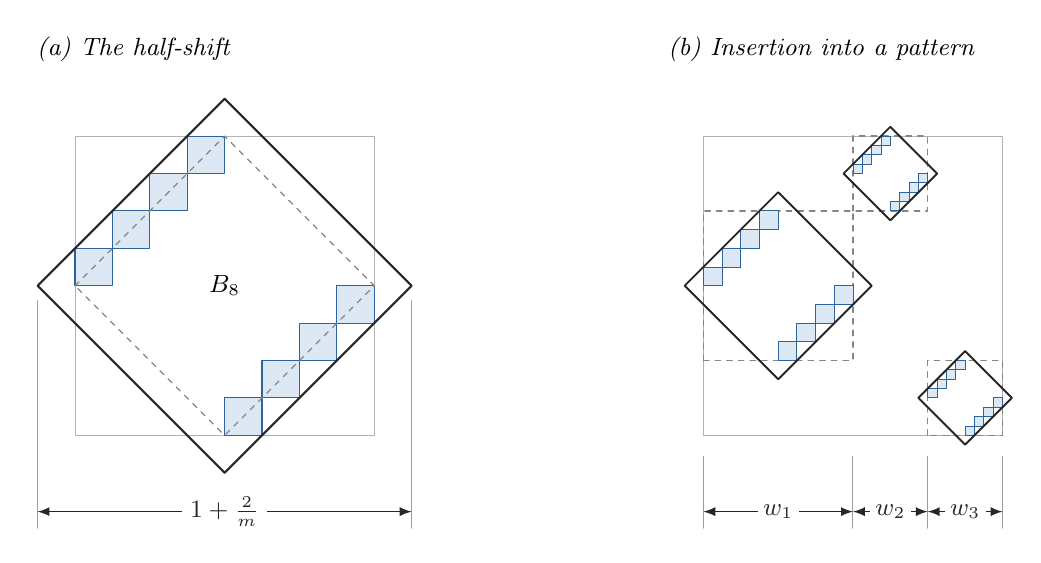
\begin{tikzpicture}[x=3.8cm,y=3.8cm,>=latex,
  every node/.style={font=\small},line cap=round,line join=round]
\node[anchor=west] at (-.16,1.29) {\textit{(a) The half-shift}};
\node[anchor=west] at (1.95,1.29) {\textit{(b) Insertion into a pattern}};

% B_8: eight squares, each of side 1/8.
\draw[black!30,line width=.35pt] (0,0) rectangle (1,1);
\foreach \i in {0,...,7}{
  \pgfmathtruncatemacro{\j}{mod(\i+4,8)}
  \path[fill=stripblue!17,draw=stripblue!85!black,line width=.4pt]
    ({\i/8},{\j/8}) rectangle ({(\i+1)/8},{(\j+1)/8});
}
\draw[black!48,dash pattern=on 2pt off 2.2pt,line width=.45pt]
  (0,.5)--(.5,1)--(1,.5)--(.5,0)--cycle;
\draw[black!85,line width=.8pt]
  (-.125,.5)--(.5,1.125)--(1.125,.5)--(.5,-.125)--cycle;
\node at (.5,.5) {$B_8$};

% An exterior dimension measures the full horizontal diameter.
\draw[black!38,line width=.35pt]
  (-.125,.45)--(-.125,-.31) (1.125,.45)--(1.125,-.31);
\draw[<->,black!85,line width=.5pt]
  (-.125,-.255)--(1.125,-.255)
  node[midway,fill=white,inner sep=3pt] {$1+\frac{2}{m}$};

% The second panel is the exact insertion of B_8 into a pattern with
% x-widths 1/2, 1/4, 1/4 and y-order 3, 1, 2.
\begin{scope}[shift={(2.10,0)}]
\draw[black!30,line width=.35pt] (0,0) rectangle (1,1);
\foreach \a/\b/\w in {0/.25/.5,.5/.75/.25,.75/0/.25}{
  \draw[black!48,dash pattern=on 2pt off 2.2pt,line width=.45pt]
    (\a,\b) rectangle ({\a+\w},{\b+\w});
  \foreach \i in {0,...,7}{
    \pgfmathtruncatemacro{\j}{mod(\i+4,8)}
    \path[fill=stripblue!17,draw=stripblue!85!black,line width=.32pt]
      ({\a+\w*\i/8},{\b+\w*\j/8})
      rectangle ({\a+\w*(\i+1)/8},{\b+\w*(\j+1)/8});
  }
  \draw[black!85,line width=.7pt]
    ({\a-\w/8},{\b+\w/2})--({\a+\w/2},{\b+9*\w/8})--
    ({\a+9*\w/8},{\b+\w/2})--({\a+\w/2},{\b-\w/8})--cycle;
}
% The side lengths visibly partition the whole unit interval.
\draw[black!38,line width=.35pt]
  (0,-.07)--(0,-.31) (.5,-.07)--(.5,-.31)
  (.75,-.07)--(.75,-.31) (1,-.07)--(1,-.31);
\foreach \a/\b/\lab in {0/.5/w_1,.5/.75/w_2,.75/1/w_3}{
  \draw[<->,black!85,line width=.5pt] (\a,-.255)--(\b,-.255)
    node[midway,fill=white,inner sep=2pt] {$\lab$};
}
\end{scope}
\end{tikzpicture}
\caption{The half-shift $B_8$ and its insertion into three squares of widths
$w_1=\frac12$, $w_2=w_3=\frac14$. The dashed diamond has diameter $1$.
The solid diamonds enclose the copies; on the right their total diameter is
$\left(1+\frac2m\right)\sum_iw_i=1+\frac2m$, with $m=8$.}
\label{fig:halfshift}
\end{figure}


Set $Q_j=B_{2j}\star P_j$.
Form the nested patterns $T_0=[0,1]^2$ and $T_j=T_{j-1}\star Q_j$.
Equations \eqref{eq:blocks}--\eqref{eq:buffer} give
\begin{equation}\label{eq:nested}
 \Fav(T_j)\le C2^{-j},\qquad \log N(T_j)\le C2^j.
\end{equation}
For the second estimate, sum the logarithmic costs of the factors:
$\sum_{i\le j}(\log(2i)+C2^i)\le C2^j$.
The factor $B_{2j}$ makes every child square at most half as wide as
its parent, so the largest square side in $T_j$ is at most $2^{-j}$.

Let $S=\bigcap_jT_j$.
The sets $v_i+w_iB_{2(j+1)}$, indexed by the squares
$v_i+w_i[0,1]^2$ of $T_j$, cover $S$.
Their diameters tend uniformly to zero, and their
total diameter is at most
$\sum_iw_i\bigl(1+\frac{1}{j+1}\bigr)=1+\frac{1}{j+1}$.
Thus $\mathcal H^1(S)\le1$.
Both coordinate projections of $S$ are $[0,1]$, by nested compactness,
so $\mathcal H^1(S)\ge1$ as well.

It remains to check the rate between successive construction scales.
Enlarging a union of $N$ squares by $[-\delta,\delta]^2$ increases
its Favard length by at most $8N\delta$: in direction $\theta$,
each projected interval gains
$2\delta(|\cos\theta|+|\sin\theta|)$.
For a fixed absolute $B>0$, equation~\eqref{eq:nested} gives
\[
 \Fav(S_\delta)\le C2^{-j}+8e^{B2^j}\delta.
\]
For small $\delta$, choose the largest $j$ with
$e^{B2^j}\le\delta^{-\frac12}$. This keeps the thickening error at most
$8\sqrt\delta$, while $2^j\asymp\log\frac1\delta$. Thus
\[
 \Fav(S_\delta)\le \frac{C}{\log\frac1\delta}+8\sqrt\delta
 \le \frac{C}{\log\frac1\delta}.
\]
The remaining values of $\delta$ are covered by increasing $C$.
Section~1 supplies the uniform marginals and the matching lower estimate,
completing the proof.
In particular, $\Fav(S)=0$ and $\mathcal H^1(S)=1$; the
Besicovitch projection theorem implies that $S$ is purely unrectifiable.

Conversely, KC2 supplies equal-grid patterns with $\A(P_j)\le2^{-j}$
and $\log N(P_j)\le C2^j$: take $n_j=\lceil\exp(C_*2^j)\rceil$.
Equations \eqref{eq:angular} and \eqref{eq:composition} give
$\Fav(P_j\star R(P_j))\le C\A(P_j)$: the two factors control the two
angular quadrants. Thus KC2 also gives \eqref{eq:blocks}, after shifting $j$ by a
fixed amount. The same half-shifts and nested insertions give Theorem~\ref{thm:favard}.
The theorem and KC2 are therefore equivalent.

\medskip
\noindent\textit{Acknowledgment.}
The main geometric idea originated with the author. Some of the more
intricate computational details were worked out with assistance from
OpenAI's Astra.

\begin{thebibliography}{9}
\bibitem{CSS}
A.~Chang, P.~Shmerkin and V.~Suomala,
\emph{Sharp Favard length of random Cantor sets},
Geom. Funct. Anal. \textbf{36} (2026), 786--830.
\href{https://doi.org/10.1007/s00039-026-00743-3}{doi:10.1007/s00039-026-00743-3}.

\bibitem{CS}
M.~Cs\"ornyei and V.~Suomala,
\emph{Which measures are projections of purely unrectifiable
one-dimensional Hausdorff measures},
Proc. Amer. Math. Soc. \textbf{137} (2009), 145--154.
\href{https://cc.oulu.fi/~vsuomala/cs.pdf}{Author manuscript}.

\bibitem{Hall}
P.~Hall, \emph{On representatives of subsets},
J. London Math. Soc. \textbf{10} (1935), 26--30.
\href{https://doi.org/10.1112/jlms/s1-10.37.26}{doi:10.1112/jlms/s1-10.37.26}.

\bibitem{Permutons}
C.~Hoppen, Y.~Kohayakawa, C.~G.~Moreira, B.~R\'ath and R.~M.~Sampaio,
\emph{Limits of permutation sequences},
J. Combin. Theory Ser. B \textbf{103} (2013), 93--113.
\href{https://doi.org/10.1016/j.jctb.2012.09.003}{doi:10.1016/j.jctb.2012.09.003}.

\bibitem{Kuklinski}
P.~Kuklinski,
\emph{An uncountable union of line segments with null two-dimensional measure},
\href{https://arxiv.org/abs/2311.16210}{arXiv:2311.16210 [math.CA]}, 2023.

\bibitem{Tao}
T.~Tao, \emph{Computing convolutions of measures},
\emph{What's new}, 26 July 2013.
\href{https://terrytao.wordpress.com/2013/07/26/computing-convolutions-of-measures/}{Online note}.
\end{thebibliography}
\end{document}
